\documentclass[11pt,a4paper]{article}

\usepackage[a4paper, top=2.5cm, bottom=2.5cm, left=2.5cm, right=2.5cm]{geometry}
\usepackage{fancyhdr}
\usepackage{booktabs}
\usepackage{array}
\usepackage{tabularx}
\usepackage{tikz}
\usetikzlibrary{calc, positioning, arrows.meta, shapes, fit, backgrounds}
\usepackage{eso-pic}
\usepackage{enumitem}
\usepackage{caption}
\usepackage{textcomp}
\usepackage{microtype}
\usepackage{hyperref}
\usepackage{xcolor}
\usepackage{amsmath}

\hypersetup{colorlinks=false,pdfborder={0 0 0}}

% Page frame on every page (drawn behind content)
\AddToShipoutPictureBG{%
  \begin{tikzpicture}[remember picture, overlay]
    \draw[line width=0.4pt]
      ([xshift=1.25cm, yshift=1.35cm]current page.south west)
      rectangle
      ([xshift=-1.25cm, yshift=-0.85cm]current page.north east);
  \end{tikzpicture}%
}

% Headers
\pagestyle{fancy}
\fancyhf{}
\fancyhead[L]{\small TruthOracle Implementation Plan}
\fancyhead[R]{\small Contract Annex}
\fancyfoot[C]{\thepage}
\renewcommand{\headrulewidth}{0.4pt}
\renewcommand{\footrulewidth}{0pt}

\setlength{\parindent}{1.5em}
\setlength{\parskip}{0.4em}

\newcolumntype{Y}{>{\raggedright\arraybackslash}X}
\newcolumntype{R}[1]{>{\raggedright\arraybackslash}p{#1}}

\begin{document}

% ---- TITLE PAGE ----
\thispagestyle{empty}
\vspace*{2cm}

\begin{center}
{\scshape Technical Implementation Plan}\\[3pt]
{\footnotesize\scshape Canton Application Layer\ \ $\vert$\ \ Prediction Markets}
\end{center}

\vspace{1.5cm}
\noindent\rule{\linewidth}{0.4pt}

\vspace{0.5cm}
\begin{center}
{\Large\bfseries TruthOracle: Technical Implementation Plan\par}
\end{center}

\vspace{0.4cm}
\noindent\rule{\linewidth}{0.4pt}

\vspace{1.5cm}
\begin{center}
\itshape
A scoped engineering plan implementing the TruthOracle protocol:\\
dynamic pm-AMM liquidity, tiered objective resolution, and the prediction-model marketplace,\\
delivered across four months with defined milestones and acceptance criteria.
\end{center}

\vspace{2cm}
\begin{center}
\begin{tabular}{r l}
\textbf{Author:} & Sachin Jangid \\[6pt]
\textbf{Prepared for:} & Cantor8 \\
\textbf{Status:}  & For Agreement (Contract Annex) \\
\textbf{Plan Version:} & 1.1 \\
\textbf{Implements:} & TruthOracle Proposal v0.6 \\
\textbf{Target SDK:} & Daml 3.4.x / Canton \\[6pt]
\textbf{Issued:} & 27 June 2026 \\
\textbf{Window:} & Weeks 1--16 (4 months from commencement) \\
\end{tabular}
\end{center}
\vfill

\newpage

% ---- 1. PURPOSE & SCOPE ----
\section{Purpose and Scope}

This document is the technical architecture and implementation plan for delivering the TruthOracle prediction market protocol as specified in the proposal it implements. It is written to be attached as an annex to a delivery agreement: it enumerates the work as discrete \textbf{workstreams}, schedules them across a \textbf{four-month} (sixteen-week) window, and binds each \textbf{milestone} to objective \textbf{acceptance criteria}. Where a behaviour is specified in the proposal, this plan references it rather than restating it.

\textbf{In scope.} Implementation of the four core Daml contracts and the optional prediction-model marketplace; the tiered resolution mechanism (T0--T3) and its off-ledger resolver/reporter services; the trading frontend and Cantor8 Enterprise Wallet integration; continuous integration, DAR build and versioning; a Canton DevNet pilot; compliance and observability tooling; a security review; and a MainNet-readiness package.

\textbf{Out of scope.} Listed explicitly in \S\ref{sec:exclusions}. In summary: regulatory licensing, the production MainNet launch itself (gated on that licensing), KYC-provider build-out, fiat on/off ramps, native mobile applications, and collateral-token issuance.

The protocol surface, contract semantics, pricing model, resolution tiers, and risk model are defined in the proposal and are not re-derived here.

% ---- 2. ARCHITECTURE OVERVIEW ----
\section{Architecture Overview}

The system is a layered application on Canton. All trust-bearing state and logic live in the Daml contract layer; off-ledger services orchestrate fetching, signing, and presentation but hold no authority the ledger does not grant them.

\begin{figure}[h]
\centering
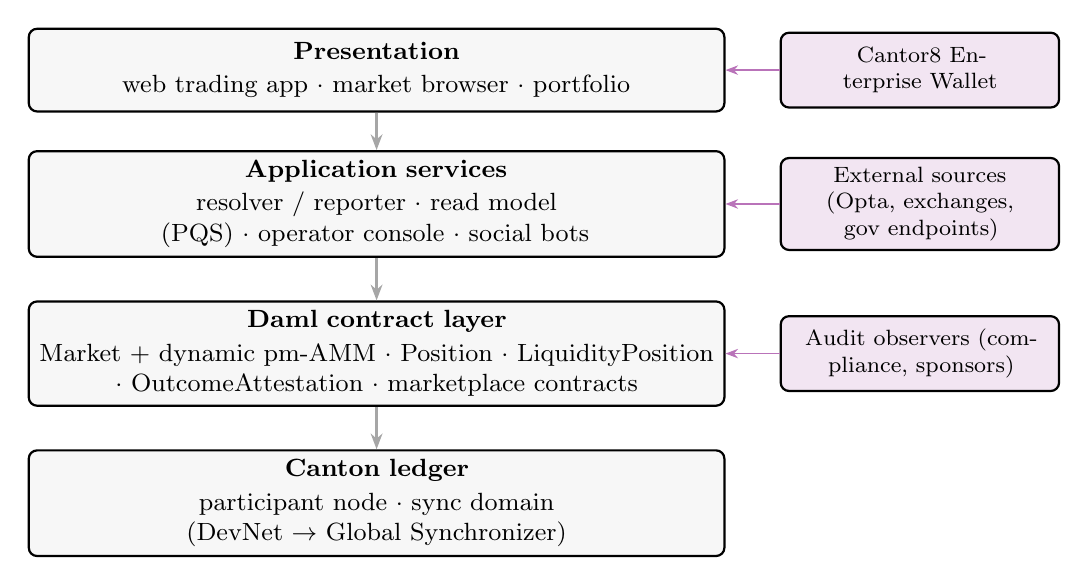
\begin{tikzpicture}[font=\small,
  layer/.style={draw, thick, rounded corners=3pt, minimum height=1.05cm,
                text width=8.6cm, align=center, fill=gray!6},
  side/.style={draw, thick, rounded corners=3pt, minimum height=0.95cm,
               text width=3.3cm, align=center, font=\footnotesize, fill=violet!10},
  flow/.style={-{Stealth[length=2mm]}, thick, gray!70},
  link/.style={-{Stealth[length=1.6mm]}, semithick, violet!55}]
\node[layer] (l1) at (-2.0,0)    {\textbf{Presentation}\\[1pt] web trading app $\cdot$ market browser $\cdot$ portfolio};
\node[layer] (l2) at (-2.0,-1.7) {\textbf{Application services}\\[1pt] resolver / reporter $\cdot$ read model (PQS) $\cdot$ operator console $\cdot$ social bots};
\node[layer] (l3) at (-2.0,-3.6) {\textbf{Daml contract layer}\\[1pt] Market + dynamic pm-AMM $\cdot$ Position $\cdot$ LiquidityPosition\\ $\cdot$ OutcomeAttestation $\cdot$ marketplace contracts};
\node[layer] (l4) at (-2.0,-5.5) {\textbf{Canton ledger}\\[1pt] participant node $\cdot$ sync domain (DevNet $\rightarrow$ Global Synchronizer)};
\draw[flow] (l1) -- (l2); \draw[flow] (l2) -- (l3); \draw[flow] (l3) -- (l4);
\node[side] (w) at (4.9,0)    {Cantor8 Enterprise Wallet};
\node[side] (s) at (4.9,-1.7) {External sources (Opta, exchanges, gov endpoints)};
\node[side] (a) at (4.9,-3.6) {Audit observers (compliance, sponsors)};
\draw[link] (w) -- (l1); \draw[link] (s) -- (l2); \draw[link] (a) -- (l3);
\end{tikzpicture}
\caption{Layered architecture. Trust resides in the Daml contract layer; the services and presentation around it are replaceable.}
\end{figure}

\noindent\textbf{Component inventory.}

\vspace{0.2em}
\begin{center}
\renewcommand{\arraystretch}{1.15}
\begin{tabularx}{\linewidth}{R{3.4cm} Y}
\toprule
\textbf{Component} & \textbf{Responsibility} \\
\midrule
Daml core package & The \texttt{Market} (with inline \emph{dynamic} pm-AMM reserves and the Gaussian pricing math --- normal-distribution $\Phi/\phi/\Phi^{-1}$, fixed-point helpers, and the invariant / optimal-reserve solver), \texttt{Position}, \texttt{LiquidityPosition}, and \texttt{OutcomeAttestation} templates, the \texttt{ResolutionPolicy} record, and shared types. \\
Resolution logic & The \texttt{Resolve}, \texttt{ProposeOutcome}, \texttt{Challenge}, \texttt{Finalize}, and \texttt{Void} choices implementing tiers T0--T3, including on-ledger \texttt{secp256k1} verification for T1. \\
Resolver / reporter service & Off-ledger service that fetches an allowlisted source over TLS, parses the outcome, signs, and creates an \texttt{OutcomeAttestation}; one instance per allowlisted reporter. \\
Read model (PQS) & Off-ledger indexer over the Participant Query Store that projects market state --- price history, volume, open interest, trade and resolution metrics, and per-market position books --- for the trading UI, dashboards, and audit observers; holds no ledger authority. \\
Operator console \& key management & Operator tooling for market creation, \texttt{ResolutionPolicy} authoring, and audit-observer administration (operator and treasury jointly), plus custody and rotation of source (T1) and reporter (T2) signing keys. \\
Marketplace package & \texttt{PredictionModel}, \texttt{ModelForecast}, \texttt{ModelPrizePool}, scoring/distribution, and the ``The Model'' aggregation. \\
Frontend \& wallet & Trading UI and Cantor8 Enterprise Wallet integration, including the two-step collateral-transfer/reconciliation flow. \\
Compliance \& observability & Audit-observer projection, position-book reporting, and operational dashboards. \\
\bottomrule
\end{tabularx}
\end{center}

% ---- 3. WORKSTREAMS ----
\section{Workstreams}

Delivery is organised into six workstreams that run partly in parallel. Each has a stable code (A--F) used throughout this plan and in the timeline.

\begin{center}
\renewcommand{\arraystretch}{1.2}
\begin{tabularx}{\linewidth}{c R{3.5cm} Y}
\toprule
\textbf{ID} & \textbf{Workstream} & \textbf{Scope} \\
\midrule
A & Core Protocol (Daml) & Implement the four core templates, the \emph{dynamic} pm-AMM pricing functions (Gaussian invariant, normal-distribution and fixed-point math, and the iterative invariant / optimal-reserve solver), and the \texttt{ResolutionPolicy}; build the Daml Script test suite covering pm-AMM invariants (price simplex, marginal price $\Phi$, value-based liquidity, time-decay $L\sqrt{T-t}$), the lifecycle, and edge cases. \\
B & Resolution Infrastructure & Implement tiers T0--T3 on-ledger and the off-ledger resolver/reporter service; onboard a test source, pin its key (T1), and configure the reporter set and quorum (T2). \\
C & Frontend \& Wallet & Build the trading frontend (market browse, buy/sell, portfolio) and integrate the Cantor8 Enterprise Wallet, including collateral transfer and reconciliation. \\
D & Deployment \& Pilot & Continuous integration, DAR build and version management, DevNet deployment, the read-model (PQS) indexer and dashboards, and operation of the pilot markets with observability. \\
E & Model Marketplace & Implement the marketplace contracts, proper-scoring distribution, the reference ``The Model'' aggregation, and a social/agent prototype. \\
F & Compliance, Security \& MainNet Readiness & Audit-observer reporting, a security review, key-management procedures, runbooks, and the MainNet go/no-go package. \\
\bottomrule
\end{tabularx}
\end{center}

% ---- 4. TIMELINE ----
\section{Implementation Timeline}

The window is sixteen weeks, grouped into four one-month phases, each closing on a review gate (G1--G4). The Gantt below shows workstream scheduling; \S\ref{sec:milestones} binds the gates to deliverables and acceptance criteria.

\begin{figure}[h]
\centering
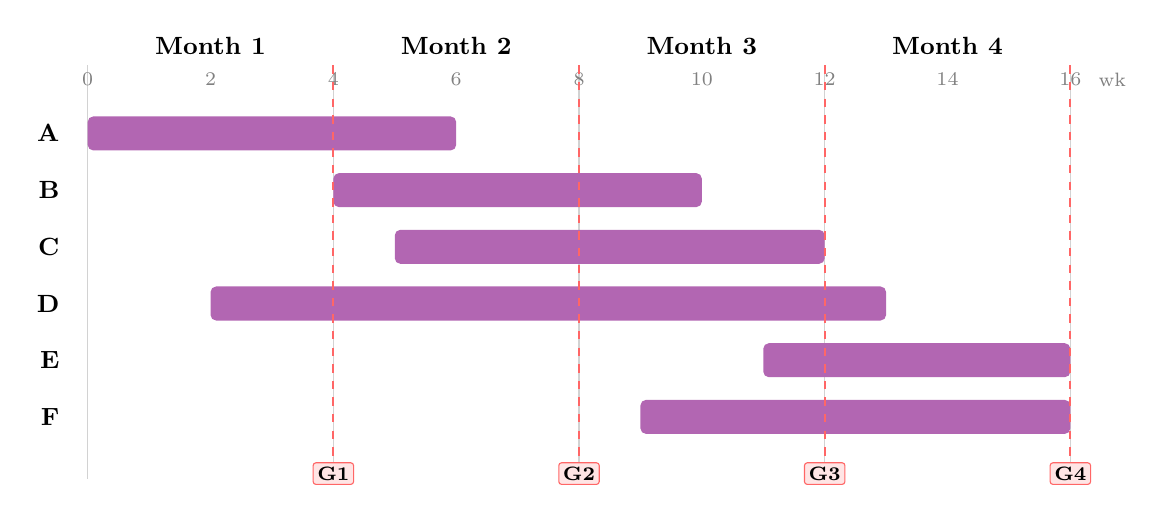
\begin{tikzpicture}[x=0.78cm, y=0.72cm]
% month gridlines
\foreach \x in {0,4,8,12,16} \draw[gray!35] (\x,0.7) -- (\x,-6.6);
% month labels
\foreach \m/\lx in {1/2,2/6,3/10,4/14} \node[font=\small\bfseries] at (\lx,1.05) {Month \m};
% week scale
\foreach \x in {0,2,4,6,8,10,12,14,16} \node[font=\scriptsize, text=gray] at (\x,0.45) {\x};
\node[font=\scriptsize, text=gray, anchor=west] at (16.3,0.45) {wk};
% rows: A..F
\foreach \row/\y/\s/\e in {A/-0.5/0/6, B/-1.5/4/10, C/-2.5/5/12, D/-3.5/2/13, E/-4.5/11/16, F/-5.5/9/16} {
  \node[anchor=east, font=\small\bfseries] at (-0.3,\y) {\row};
  \draw[fill=violet!60, draw=none, rounded corners=2pt] (\s,\y-0.3) rectangle (\e,\y+0.3);
}
% gate markers
\foreach \g/\x in {G1/4, G2/8, G3/12, G4/16} {
  \draw[red!60, thick, dashed] (\x,0.7) -- (\x,-6.2);
  \node[draw=red!60, fill=red!10, font=\scriptsize\bfseries, inner sep=1.5pt, rounded corners=1pt] at (\x,-6.5) {\g};
}
\end{tikzpicture}
\caption{Sixteen-week schedule. A Core Protocol, B Resolution Infrastructure, C Frontend \& Wallet, D Deployment \& Pilot, E Model Marketplace, F Compliance/Security/MainNet Readiness. Gates G1--G4 close each month.}
\end{figure}

\subsection*{Month 1 (Weeks 1--4) --- Core Protocol \& Tier 0}
Stand up the repository, CI, and DAR build (WS-D). Implement the Daml core package and \emph{dynamic} pm-AMM pricing --- the Gaussian invariant, normal-distribution and fixed-point approximations, and the iterative solver (WS-A) --- and the Tier-0 designated-operator resolution path (WS-B). Produce the Daml Script test suite for pm-AMM invariants and the full lifecycle. \emph{Closes at G1.}

\subsection*{Month 2 (Weeks 5--8) --- Resolution Tiers \& Frontend MVP}
Implement T1 (first-party \texttt{secp256k1} verification), T2 (reporter quorum), and T3 (optimistic propose/challenge/finalize with bonds) on-ledger, plus the off-ledger resolver/reporter service (WS-B). In parallel, build the frontend MVP and Cantor8 wallet integration (WS-C). \emph{Closes at G2.}

\subsection*{Month 3 (Weeks 9--12) --- DevNet Pilot}
Deploy the DAR to Canton DevNet under \texttt{TruthOracle::devnet} and operate three pilot markets --- one T0, one T2 (2-of-3 reporters), one T3-over-T2 (WS-D). Stand up audit-observer projection, position-book reporting, and dashboards (WS-F). Track pilot KPIs. \emph{Closes at G3.}

\subsection*{Month 4 (Weeks 13--16) --- Marketplace \& MainNet Readiness}
Implement the prediction-model marketplace contracts, proper-scoring distribution, the ``The Model'' aggregation, and a social/agent prototype (WS-E). Conduct the security review, document resolver/source key management, and assemble the MainNet runbooks and go/no-go package (WS-F). \emph{Closes at G4.}

% ---- 5. MILESTONES & DELIVERABLES ----
\section{Milestones, Deliverables, and Acceptance Criteria}
\label{sec:milestones}

Each gate is met when all of its deliverables satisfy their acceptance criteria, verified against the in-memory IDE ledger and the persistent Canton sandbox (or DevNet, where stated).

\renewcommand{\arraystretch}{1.25}

\noindent\textbf{Gate G1 --- Core Protocol \& Tier 0 (end of Week 4)}
\begin{center}
\begin{tabularx}{\linewidth}{c R{4.2cm} Y}
\toprule
\textbf{ID} & \textbf{Deliverable} & \textbf{Acceptance criterion} \\
\midrule
D-A1 & Daml core package & Compiles on Daml SDK 3.4.x; produces a versioned DAR with a stable package \texttt{name}. \\
D-A2 & Dynamic pm-AMM \& lifecycle test suite & Daml Script tests pass for the Gaussian price-simplex invariant ($P=\Phi((y-x)/L_{\mathrm{eff}})$), time-decay $L_{\mathrm{eff}}=L\sqrt{T-t}$, value-based liquidity, buy/sell, and the create$\rightarrow$trade$\rightarrow$resolve$\rightarrow$redeem lifecycle. \\
D-B1 & Tier-0 resolution path & Operator can resolve a market from a designated source and a holder can redeem; void path verified. \\
D-D1 & CI \& DAR versioning & Automated build/test on every change; version bump publishes a successor DAR recognised as an in-place upgrade. \\
\bottomrule
\end{tabularx}
\end{center}

\noindent\textbf{Gate G2 --- Resolution Tiers \& Frontend MVP (end of Week 8)}
\begin{center}
\begin{tabularx}{\linewidth}{c R{4.2cm} Y}
\toprule
\textbf{ID} & \textbf{Deliverable} & \textbf{Acceptance criterion} \\
\midrule
D-B2 & T1 first-party signature & A correctly signed payload resolves the market; a tampered payload or wrong key is rejected on-ledger via \texttt{secp256k1}. \\
D-B3 & T2 reporter quorum & $M$-of-$N$ agreeing attestations resolve; disagreement or sub-quorum does not resolve and the market can be voided after grace. \\
D-B4 & T3 optimistic flow & An unchallenged proposal finalizes after the window; a challenge escalates to T1/T2 and the losing bond is slashed to the winner. \\
D-B5 & Resolver/reporter service & Service fetches a test source over TLS, parses, signs, and creates a valid \texttt{OutcomeAttestation}; runs one instance per reporter. \\
D-C1 & Frontend MVP & Browse markets, execute buy/sell through the pm-AMM, and view positions on the sandbox. \\
D-C2 & Wallet integration & Connect the Cantor8 Enterprise Wallet; collateral transfer and reconciliation complete for buy/sell. \\
\bottomrule
\end{tabularx}
\end{center}

\noindent\textbf{Gate G3 --- DevNet Pilot (end of Week 12)}
\begin{center}
\begin{tabularx}{\linewidth}{c R{4.2cm} Y}
\toprule
\textbf{ID} & \textbf{Deliverable} & \textbf{Acceptance criterion} \\
\midrule
D-D2 & DevNet deployment \& pilot markets & DAR deployed under \texttt{TruthOracle::devnet}; three markets live (T0; T2 2-of-3; T3-over-T2). \\
D-D3 & Observability \& dashboards & Trade and resolution metrics are visible; pm-AMM invariant integrity is independently checkable. \\
D-F1 & Compliance reporting & A designated audit observer can retrieve the full position book for its market(s). \\
--- & Pilot KPIs (tracked) & Progress toward $\geq 90$ distinct trader parties, $\geq 500$ \texttt{Buy} transactions, and zero failed-resolution incidents. \\
\bottomrule
\end{tabularx}
\end{center}

\noindent\textbf{Gate G4 --- Marketplace \& MainNet Readiness (end of Week 16)}
\begin{center}
\begin{tabularx}{\linewidth}{c R{4.2cm} Y}
\toprule
\textbf{ID} & \textbf{Deliverable} & \textbf{Acceptance criterion} \\
\midrule
D-E1 & Marketplace contracts \& scoring & Forecasts commit only while a market is open; Brier scoring and pool distribution are tested and reproducible by an audit observer. \\
D-E2 & ``The Model'' \& social prototype & A reference forecast is published; a bot posts market state to a test social channel. \\
D-F2 & Security review \& key management & Review report delivered with findings triaged; resolver/source key custody and rotation documented. \\
D-F3 & MainNet readiness package & Deployment runbook, rollback procedure, and a go/no-go checklist are delivered (execution gated on external licensing). \\
\bottomrule
\end{tabularx}
\end{center}

% ---- 6. DEPENDENCIES ----
\section{Dependencies and Assumptions}

\textbf{External dependencies.}
\begin{itemize}[leftmargin=2em, itemsep=2pt]
\item CIP-56 token semantics available on the target network for collateral denomination.
\item Access to the Cantor8 Enterprise Wallet SDK and a test wallet environment.
\item Canton DevNet access and allocation of the \texttt{TruthOracle::devnet} operator party.
\item A test data source for resolution (e.g., an Opta sandbox/test feed) and, for T1, a signing arrangement that publishes a pinnable public key.
\item Nomination of the independent reporter parties used for T2 quorum during the pilot.
\end{itemize}

\textbf{Assumptions.}
\begin{itemize}[leftmargin=2em, itemsep=2pt]
\item Target platform is Daml SDK 3.4.x on Canton; \texttt{DA.Crypto.Text} (\texttt{sha256}, \texttt{secp256k1}) is available in the standard library.
\item Daml \texttt{Decimal} (38-digit fixed precision) is sufficient for the dynamic pm-AMM normal-distribution approximations and invariant solver; no external numerical library is required.
\item The team is staffed per \S\ref{sec:resourcing} for the full window.
\item DevNet and the test source feeds are reasonably available through Month 3.
\item Regulatory licensing proceeds on a separate, parallel track owned by Cantor8.
\end{itemize}

% ---- 7. RISK REGISTER ----
\section{Risk Register}

\renewcommand{\arraystretch}{1.2}
\begin{center}
\begin{tabularx}{\linewidth}{Y c c Y}
\toprule
\textbf{Risk} & \textbf{Impact} & \textbf{Likely} & \textbf{Mitigation} \\
\midrule
Data source cannot sign (T1 unavailable) & Med & Med & Fall back to T2 reporter quorum, which needs nothing of the source; pursue T1 signing as an enhancement. \\
DevNet instability or downtime & Med & Med & Develop against the local sandbox; treat DevNet as a deployment target, not a development dependency. \\
Cantor8 wallet SDK access delayed & High & Low & Build C against a mock wallet adapter behind an interface; swap in the real SDK without UI rework. \\
Reporter parties not nominated in time & Med & Med & Run the pilot's T2 market with internal reporters first; substitute independent parties before MainNet. \\
Scope creep from new market types & Med & Med & Hold scope to binary markets per the proposal; log scalar/multi-outcome as a follow-on. \\
Dynamic pm-AMM numerical precision / solver convergence in Daml \texttt{Decimal} & Med & Low & Optimal reserves, liquidity sizing, and pool value are \emph{closed-form} in price ($x^*,y^*,V$ via $\Phi^{-1}$); only the swap direction needs a guarded one-dimensional root find. Use vetted rational approximations for $\Phi/\phi/\Phi^{-1}$ with bounded error; property-test invariants and pin tolerances; fall back to a coarser static-$L$ profile at precision limits. \\
Security review surfaces blocking findings & High & Low & Schedule the review early in Month 4 with buffer; triage and fix critical findings before G4. \\
Licensing slips (external) & High & Med & Engineering delivers a MainNet-ready package at G4; launch decoupled and gated on Cantor8's licensing track. \\
\bottomrule
\end{tabularx}
\end{center}

% ---- 8. TEAM ----
\section{Team and Resourcing}
\label{sec:resourcing}

The plan is delivered by a two-person senior team across the window:

\begin{itemize}[leftmargin=2em, itemsep=2pt]
\item \textbf{Lead Engineer} --- owns the Daml core protocol and resolution (WS-A, WS-B), the off-ledger resolver/reporter service, continuous integration and DevNet deployment (WS-D), and the security review and compliance reporting (WS-F). Accountable for the gate deliverables.
\item \textbf{Full-Stack Engineer} --- owns the trading frontend and Cantor8 wallet integration (WS-C) and the prediction-model marketplace and social/agent prototype (WS-E), and builds the observability dashboards within WS-D.
\end{itemize}

The two engineers share WS-D and WS-F operationally; all backend and service work is absorbed into these two roles. Should Cantor8 wish, an independent security reviewer may be commissioned for WS-F, but the plan does not assume one.

Cantor8 provides the wallet SDK, DevNet access and party allocation, data-source and reporter introductions, and the business/compliance counterpart for gate reviews.

% ---- 9. REVIEW CADENCE ----
\section{Review Cadence and Governance}

\begin{itemize}[leftmargin=2em, itemsep=2pt]
\item \textbf{Bi-weekly demo} --- a working build is demonstrated every two weeks against the sandbox or DevNet.
\item \textbf{Monthly gate review (G1--G4)} --- at each gate, deliverables are checked against their acceptance criteria and signed off jointly before the next phase begins. A gate not met is re-scoped at the review rather than silently carried forward.
\item \textbf{Change control} --- scope changes are recorded against this annex with their schedule impact, so the agreement and the plan stay consistent.
\end{itemize}

% ---- 10. EXCLUSIONS ----
\section{Exclusions (Out of Scope)}
\label{sec:exclusions}

The following are explicitly outside this engagement and are noted so the agreement is unambiguous:

\begin{itemize}[leftmargin=2em, itemsep=2pt]
\item Regulatory licensing in any jurisdiction, and the production MainNet launch, which is gated on that licensing.
\item Build-out of a KYC/AML provider; the plan integrates with Cantor8's existing arrangements rather than building one.
\item Fiat on/off ramps and collateral-token issuance.
\item Native mobile applications (the frontend is web).
\item Formal verification or a full external audit beyond the scoped Month-4 security review.
\item New market structures beyond binary markets (e.g., scalar or multi-outcome), which are a follow-on per the proposal.
\end{itemize}

\bigskip
\noindent\textbf{Document control}

\smallskip
\textit{Plan v1.1 (27 June 2026).} Four-month technical implementation plan implementing TruthOracle proposal v0.6, revised for the dynamic pm-AMM, the read-model (PQS) indexer, and the operator-console / key-management control plane; for attachment to the delivery agreement. (v1.0, 10 June 2026: initial plan.)

\bigskip
\noindent\textbf{Copyright}

This document is licensed under the Apache License, Version 2.0.

\end{document}
